\documentclass[a4paper,10pt]{article}
\usepackage{geometry}
 \geometry{ a4paper, total={170mm,257mm}, left=20mm, top=20mm}
\usepackage{verbatim}
\usepackage[utf8]{inputenc}
\usepackage{amsmath}
%\usepackage{gensymb}
\usepackage{verbatim} % env for block comment 
\usepackage{ragged2e} % para usar flusleft
\usepackage[brazilian]{babel}
\usepackage{hyperref}
\usepackage{array}
\usepackage{multirow}
\usepackage{tabu}
\usepackage{booktabs}
\usepackage{parskip}
\hypersetup{
    colorlinks=true,
    linkcolor=red,
    filecolor=magenta,      
    urlcolor=blue,
    pdftitle={zrhans@gmail.com},
    %bookmarks=true,
    pdfpagemode=FullScreen,}
    
\urlstyle{same}
\usepackage{minted}     % Realce de código
\usemintedstyle{tango}  % Tema do realce de código

\usepackage{wrapfig}
\usepackage[export]{adjustbox} % Ajuste das imagens To change the default alignment of a image from left or right 

\usepackage{tikz,tkz-euclide}
\usepackage{circuitikz} 


\usepackage{fancyhdr}
 
\pagestyle{fancy}
\fancyhf{}
\renewcommand{\headrulewidth}{2pt}
\renewcommand{\footrulewidth}{1pt}
\rhead{\href{http://portalfisica.com}{portalfisica.com}}
\lhead{UFSM}
\lfoot{Prof. Hans R. Zimermann - hans@ufsm.br}
\rfoot{Página - \thepage}

\begin{document}

\begin{wrapfigure}{l}{0.2\textwidth}

\includegraphics[width=.7\linewidth]{img/atm} 
\end{wrapfigure}

\noindent
\textsc{UFSM00029 - Física Experimental III \\ FSC1026 - Física Geral Experimental III \\ FSC326  \, -  Laboratório de Física III} \\
Engenharias e Física \\
Semestre - 1.2023 \\
Prof. Hans R. Zimermann \\

\noindent \rule{\linewidth}{0.5mm}

\begin{flushright}
{\color{orange}\textit{\mbox{"A perfeição é atingida não quando não se tem mais o que colocar,} \\ \mbox{ mas sim quando não se tem mais o que tirar." \;- Antoine de Saint-Exupéry}} }
\end{flushright}

%%%%%%%%%%%%%%%%%%%%%%%%%%%%%%%%%%%%%%%
%                PARTES
%%%%%%%%%%%%%%%%%%%%%%%%%%%%%%%%%%%%%%%

\noindent \texttt{V: 24-03-2023 23:16:00}

\section*{Experimento: - Máquinas Eletrostáticas - Gerador Van De Graaff}

\section*{Teoria}
\subsection*{Introdução}

\begin{wrapfigure}{R}{0.3\textwidth}
\centering
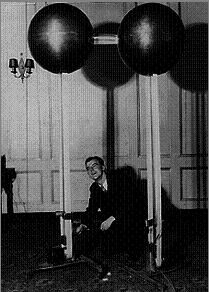
\includegraphics[width=0.7\linewidth]{img/rj-vandegraaff.png} 
	\caption{Robert J. Van de Graaff e uma das primeiras versões do Gerador Van de Graaff \textit{Fonte: http://www.cmm.gov.mo}.}
	\label{fig:robert-j-vgraaff}
\end{wrapfigure}
Por volta de 1930, o engenheiro estado-unidense Robert Jeminson Van de Graaff inventou uma 
máquina capaz de demonstrar de forma visível a ação da eletricidade a partir da transferência das 
cargas elétricas de um corpo eletrizado para outro. Em sua homenagem, esse aparelho foi batizado
de Gerador de Van de Graaff. Seus princípios ainda são utilizados atualmente, a máquina atua na 
física nuclear, em versões mais potentes, para produzir tensões muito elevadas em aceleradores de 
partículas, assim como na medicina e na indústria de alta tecnologia.

\noindent Essa máquina será fundamental para atingir o objetivo do experimento que será realizado em 
laboratório. Sob instruções do Professor, a turma de Física Experimental III
utilizará o Gerador de Van de Graaff para executar três procedimentos em laboratório e 
verificar as manifestações da força elétrica e o comportamento das cargas estáticas submetidas à 
situações de transferência de cargas entre dois corpos, bem como para analisar a disposição dessas 
cargas de acordo com o formato de cada corpo e seus efeitos resultantes.

\subsection*{Fundamentos da Eletrostática e Gerador Van De Graaff}
Os fundamentos básicos da eletrostática regem o funcionamento do Gerador de Van de Graaff, 
sendo eles: o Princípio da atração e repulsão, responsável por demonstrar que cargas de mesmo 
sinal tendem a se repelir e cargas de sinais contrários tendem a se atrair. O Princípio da conservação 
de cargas, o qual define que a quantidade total de cargas de um sistema é sempre constante. E os 
tipos de eletrização (Atrito, Contato e Indução) que definem como acontece a transferência das 
cargas. De maneira geral, pode-se dizer o gerador auto-excitado funciona de acordo com os princípios do \textbf{efeito tribolelétrico}, se referindo ao fenômeno que ocorre quando dois materiais de composição diferentes estão bem juntos e então são puxados de maneira que se separem num curto intervalo de tempo.

O gerador de Van de Graaff funciona através da movimentação de uma correia que é eletrizada por 
atrito na parte inferior do aparelho. Ao atingir a parte superior, as cargas elétricas que surgiram com o processo de eletrização por Atrito, são transferidas para a superfície interna do metal, sendo então 
distribuídas para toda a superfície da esfera metálica, ficando carregada de cargas elétricas. Se durante o funcionamento do gerador aproximarmos o dedo ou um objeto de metal perceberemos leves descargas elétricas que ocorrem em razão da diferença de potencial. 
De maneira geral, esse gerador é composto por:

\begin{itemize}
    \item  Um motor; 
    \item  Dois cilindros (um condutor e outro isolante); 
    \item  Um conjunto de correias; 
    \item  Um conjunto de escovas; 
    \item  Um terminal de saída, que na maioria das vezes é uma grande esfera metálica ou recoberta por um material condutor.
\end{itemize}



\section*{Prática}
\section{Objetivos}
\begin{itemize}
    \item[i] Verificar comportamento de cargas estáticas e as manifestações da Força Elétrica;
    \item[ii] Faça a revisão bibliográfica sobre o assunto: "Fundamentos da eletrostática e do Gerador de Van De Graaff";
    \item[iIi] Faça algumas imagens do experimento.
\end{itemize}

\section{Material Utilizado}
\begin{itemize}
    \item Gerador Van De Graaff
    \item Eletroscópio
    \item Condutores Pontiagudos (Lança, Torniquete)
    \item Vela
    \item Lâmpadas de Gazes diversos (Ionização e DDP)
    \item Diversos fios condutores e acessórios
\end{itemize}
\par 
\noindent oi

\section{Procedimento experimental}
Realizar três experimentos para observar o comportamento das cargas elétricas, sendo eles:

\begin{itemize}
    \item  Força Elétrica - Eletroscópio
    \item  Poder das Pontas - “Para-raios”
    \item  Vento Iônico
\end{itemize}

\subsection{Força elétrica – Eletroscópio:}

\subsubsection{FUNÇÃO:}

\noindent Esse experimento teve a função de verificar se um corpo está ou não eletrizado, assim como observar a intensidade da sua eletrização

\subsubsection{MATERIAIS UTILIZADOS:} 
\begin{itemize}
    \item[a)] Gerador de Van de Graaff
    \item[b)] Material isolante
    \item[c)] Fios condutores
    \item[d)] Eletroscópio
    \item[e)] Corpo condutor que será eletrizado
\end{itemize}

\subsubsection{PROCEDIMENTO:} 
Ligou-se o Gerador de Van de Graaff na corrente elétrica, a qual fez a correia movimentar-se entre as escovas, eletrizando-a por atrito. As cargas negativas chegaram até a esfera de alumínio por contato.

\noindent Com o gerador eletrizado, aproximou-se uma outra esfera condutora, a qual teve suas cargas separadas por Indução. Após isso, ligou-se a parte positiva da esfera na terra para descarregar as cargas e o corpo também ficar eletrizado negativamente
Sob essas condições, foi possível observar a repulsão das cargas nas extremidades do eletroscópio, quando aproximado de algum dos corpos. Informando-nos que o corpo estava eletrizado.

\subsection{Poder das pontas – “Para-raios”}

\subsubsection{FUNÇÃO:}
Esse experimento teve a função de verificar a distribuição das cargas elétricas em um corpo que 
possui extremidades pontiagudas
\subsubsection{MATERIAIS UTILIZADOS: }
\begin{itemize}
    \item[a)] Gerador de Van de Graaff
    \item[a)] Fios condutores
    \item[a)] Lança pontiaguda
\end{itemize}

\subsubsection{PROCEDIMENTO:}
Antes de ligar o Gerador de Van de Graaff na corrente elétrica, posicionou-se a lança pontiaguda no topo da esfera metálica.

\noindent Assim que o Gerador começou a funcionar, percebeu-se que não houve acúmulo considerável de cargas na superfície da esfera oca, em comparação com os procedimentos anteriores. Em contrapartida, havia grandes concentrações de carga ao redor da lança pontiaguda. Isso deve-se ao princípio do “Poder das Pontas”, que define que as cargas elétricas de um corpo se concentram nas regiões mais pontiagudas, fazendo com que o campo elétrico nas vizinhanças 
dessas pontas atinja determinado valor, ionizando o ar em sua volta, tornando-o condutor. Esse princípio é utilizado nos para-raios, fazendo com que a nuvem eletrizada descarregue suas cargas nas pontas do para-raio. Como o para-raio está ligado a terra, as cargas elétricas recebidas são transferidas ao solo sem nenhum problema. 

\subsection{Vento Iônico}
\subsubsection{FUNÇÃO:}
Esse experimento teve a função de observar a repulsão das cargas elétricas gerada pela ionização 
do ar.
\subsubsection{MATERIAIS UTILIZADOS: }
\begin{itemize}
    \item[a)] Gerador de Van de Graaff
    \item[a)] Fios condutores
    \item[a)] Lança pontiaguda
    \item[a)] Torniquete com 4 pontas em forma de “Z”
    \end{itemize}
    
\subsubsection{PROCEDIMENTO: }
Antes de ligar o Gerador de Van de Graaff na corrente elétrica, posicionou-se a lança pontiaguda no topo 
da esfera metálica com o torniquete conectado à ponta da lança pontiaguda. 
Quando o gerador for ligado na corrente elétrica, deve se observar que o torniquete começará a girar. 
Esse efeito deve-se à ionização do ar nas pontas do torniquete, a qual concentrou as cargas 
devido ao “Poder das pontas” e gerou repulsão dos íons de mesmo sinal, determinando a rotação 
acelerada nas pontas. 


\begin{thebibliography}{9}

\bibitem{jeewett11}
  JEWETT JR, J.W., SERWAY, R. A. 
  \emph{Física para cientistas e engenheiros: Eletricidade e magnetismo},
  CENGANGE Learning,
  São Paulo:
  2011

\bibitem{halliday3}
David Halliday, Robert Resnick, Jearl Walker; \emph{F Fundamentos de Física, Volume 3}, 8ª edição, São Paulo 2010. 
 
\bibitem{juraitis}
JURAITIS, K. R.; DOMICIANO, J. B.; \emph{Capítulo 1 - O Laboratório de Física - Introdução ao Laboratório de Física Experimental}, Londrina, PR, 2009

\bibitem{coeufrj}
COE UFRJ 
\emph{Máquinas Eletrostáticas}, \\ \url{www.coe.ufrj.br/~acmq/eletrostatica.html} -  - Acesso em 23/03/2023

\bibitem{jifufrgs}
IF UFRGS - Instituto de Física - UFRGS
\emph{Circuitos Elétricos}, \\ \url{www.if.ufrgs.br/tex/fis142/mod07/m\_s02.html} - Acesso em 01/05/2017

\bibitem{ifscusp}
IFSC USP
\emph{Gerador eletrostático Van De Graaff}
\\ \url{www.ifsc.usp.br/~strontium/Teaching/Material2010-2\%20FFI0106\%20LabFisicaIII/App01b\%20Eletrostatica.pdf} - Acesso em 24/03/2023.

\bibitem{yumpu}
Projeto para Feira do Saber \emph{Tema: Gerador eletrostático de Van dde Graaff} - 
\\ \url{https://www.yumpu.com/pt/document/read/12806191/gerador-eletrostatico-de-van-de-graaffpdf-colegio-decisao} - Acesso em 25/03/2023.
  
\end{thebibliography}

%\noindent \texttt{V: 25-10-2022 17:28:00}
\section*{Experimento: - CAPACITÂNCIA}
	\section{Objetivos}
	
	Estudar o efeito capacitivo entre as placas de um capacitor variável de placas paralelas - Figura \ref{fig:cidepe-capacitor}, verificando a relação da capacitância $C=\epsilon_{0} A/d$ em função da distância $d$ entre as placas; Medir a constante de permissividade ${\epsilon}_{0}$ e medir a constante dielétrica de distintos materiais isolantes como papel, \href{https://pt.wikipedia.org/wiki/Espuma_vin\%C3\%ADlica_acetinada}{ E.V.A (\textit{Ethylene Vinyl Acetate})} e isopor.	
	\section{Material utilizado}
	
\begin{wrapfigure}{r}{0.7\textwidth}
    \centering
    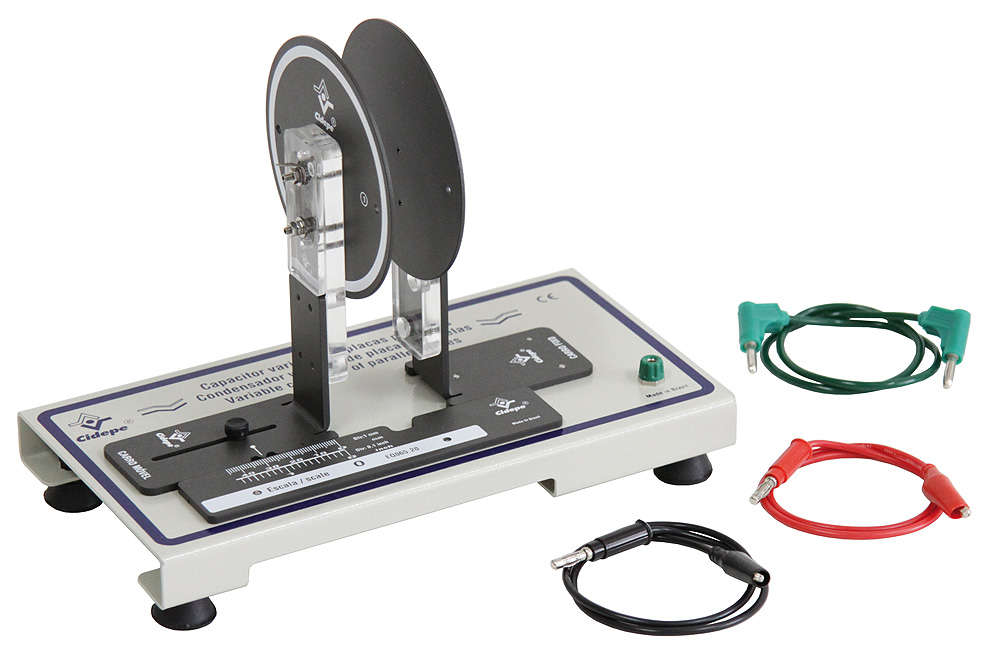
\includegraphics[width=.36\textwidth]{img/cidepe-capacitor.jpg}
    \caption{Capacitor de placas paralelas com separação variável montado em isolante acrílico. \textit{Fonte: Cidepe}.}
    \label{fig:cidepe-capacitor}
\end{wrapfigure}
	
	\begin{itemize}
		\item[a)] Um capacitor variável de placas paralelas: 2,3 pF - 280 pF;
		\item[b)] Um medidor digital de capacitância;
		\item[c)] Dois fios ou cabos condutores;
		\item[d)] Um papel milimetrado;
		\item[e)] Folhas de papel ou papelão;
		\item[f)] Lâminas de isolantes E.V.A, EPS (Isopor), Vidro, Acrílico,etc;
		\item[j)] Uma régua ou trena ou paquímetro.
		
	\end{itemize}
	
\begin{comment}
\begin{figure}[H]
	\centering
	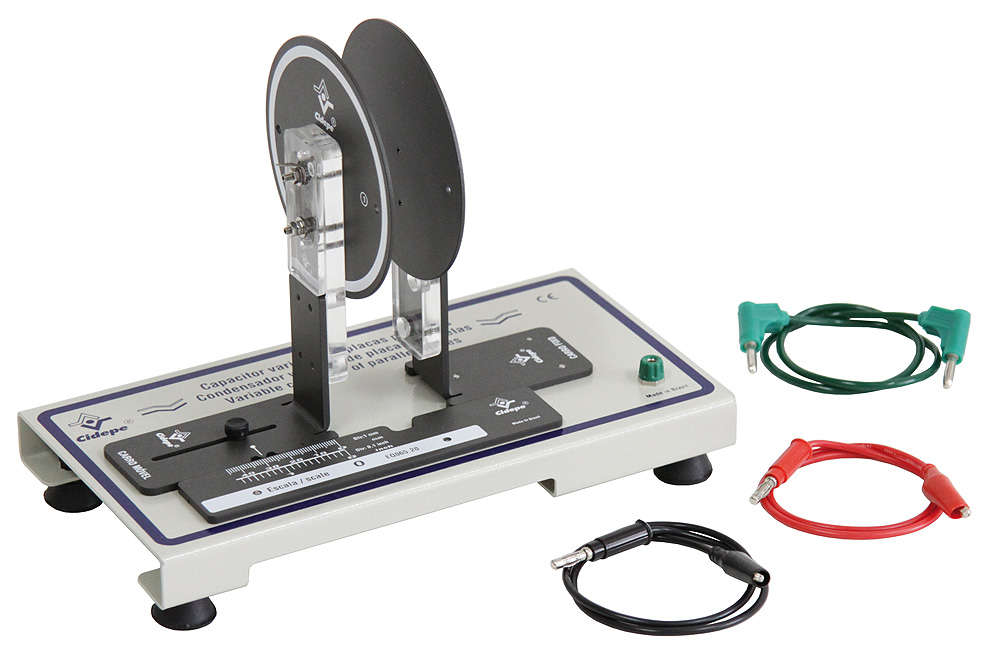
\includegraphics[scale=.3]{img/cidepe-capacitor.jpg}
	\caption{Capacitor de placas paralelas com separação variável montado em isolante acrílico. Fonte: Cidepe.}
	\label{fig:imagem1}
\end{figure}
\end{comment}


\section{Fundamentos teóricos}
	
	Se preenchermos o espaço entre as placas de um capacitor com um dielétrico (isolante), o que acontecerá com a capacitância? \textbf{Michel Faraday} (1791-1867) investigou este assunto pela primeira vez em 1837. Usando equipamento simples, ele descobriu que a capacitância aumentava por um fator $\kappa$, que ele chamou de constante dielétrica do material isolante. Outro efeito importante na introdução do dielétrico no capacitor é limitar a diferença de potencial que se pode aplicar entre as placas a um certo valor ${V}_{max}$, chamado de potencial de ruptura. Se este valor for excedido, o material dielétrico se romperá e formará um caminho condutor ({\color{red}\textbf{arco elétrico}}) entre as placas. Logo, todo material dielétrico possui uma rigidez dielétrica característica, que é o valor máximo do campo elétrico que um isolante pode tolerar sem se romper e se tornar um condutor (para o ar a rigidez dielétrica é $~3\times10^{6} \,V.m^{-1}$, ou seja tensões ou diferenças de potencial ${V}_{max}$ acima desses valores, permitem a ocorrência de um \textbf{arco elétrico} ou popularmente \textit{raio/faísca/centelha}). Na Tabela \ref{tab:rigidez-materiais} são mostradas algumas constantes dielétricas importantes.
	
	%tabela 1
	\begin{table}[H]
		\centering
	\begin{tabular}{l|c|c}
		\hline 
		Material & Constante Dielétrica, $\kappa$ & Rigidez Dielétrica $E_{max} (10^{6}\,V.m^{-1})$ \\ 
		\hline 
		Ar(1 atm) & 1,0006 & 3 \\ 
        Madeira & & 10 \\
        Borracha & & 12 \\
	Papel & 3,5 & 16 \\ 
        Poliéster & 3,6 & 21,7 \\ 
        Vidro & & 30 \\
        Mica & & 60 \\
        Teflon & & 80 \\
        
		\hline 
	\end{tabular} 
		\caption{Constante dielétrica e rigidez dielétrica}
		\label{tab:rigidez-materiais}
	\end{table}

	\section{Procedimento experimental}
	
	\subsection{A - MEDIDA DA PERMISSIVIDADE ELÉTRICA ($\epsilon_{0}$)}
	
	\begin{itemize}
		\item[a)] Certifique-se de que o capacitor esteja descarregado, fazendo contato entre as duas placas por meio de um fio ou cabo condutor;
		\item[b)] Meça o diâmetro, calcule o raio e com este a área das placas do capacitor (use: $A=\pi r^2$, onde $r$ é o \textbf{raio} das placas). Anote os resultados na Tabela \ref{tab:area-placas};
		
		%tabela 2
		\begin{table}[H]
			\centering
		\begin{tabular}{|c|c|}
			\hline 
			Diâmetro das Placas ($m$) & Área das Placas do Capacitor ($m^2$)\\ 
			\hline
			&  \\ 
			\hline 
		\end{tabular}
			\caption{\label{tab:area-placas} Diâmetro e área do capacitor}
		\end{table}
		
		\item[c)] Fazer a conexão do medidor de capacitância nas placas do capacitor. \textbf{Zerar o aparelho antes de fazer a medida};
		\item[d)] Com a chave seletora do medidor em 200 pF, estabeleça um espaçamento aproximado de 1,0 ou 10 mm entre as placas do capacitor. Anote o valor da capacitância $C_{exp}$ na Tabela \ref{tab:cte-dieletrica}; 
		\item[e)] Calcule a constante de permissividade (use a relação: $ \epsilon_{0}= C_{exp} \, d / A. \kappa_{ar} $). Anote o resultado na Tabela \ref{tab:cte-dieletrica};
		\item[f)] Calcule o erro experimental, entre o valor teórico (da literatura), e o valor experimental (medido). Anote o resultado na Tabela \ref{tab:cte-dieletrica}. 
	
		%tabela 3
		\begin{table}[H]
			\centering
		\begin{tabular}{|c|c|c|c|c|}
			\hline 
			$C_{exp}$ (pF) & $\epsilon_{0}$ (Teórico)(pF) & $\epsilon_{0}$ (experimental)(pF) & Erro (Absoluto) & Erro (\%)  \\ 
			\hline 
			& 8,85 & & & \\ 
			\hline 
		\end{tabular}
			\caption{Medição da constante dielétrica}
			\label{tab:cte-dieletrica}
		\end{table} 
	\end{itemize}
	
	\subsection{B - VARIAÇÃO DA CAPACITÂNCIA COM A SEPARAÇÃO ENTRE AS PLACAS}
	
	\begin{itemize}
		\item[a)] Certifique-se de que o capacitor esteja descarregado;
		\item[b)] Com a chave seletora do medidor em 200 pF, varie a distância entre as placas de 1 mm em 1 mm até 10 mm (5 mm em 5 mm até 50 mm no Capacitor \href{https://www.cidepe.com.br/index.php/br/produtos-interna/capacitor-variavel-de-placas-paralelas-e-cabos-0-a-255-pf-1875}{Cidepe EQ065D} ou similar). Para cada variação meça a capacitância correspondente ({\color{red}\textbf{Para uma melhor precisão, a partir da segunda medida selecione a posição da chave em $200 \,\mu F$}}). Anote os valores das capacitâncias $ C_{exp} $ na Tabela \ref{tab:c-versus-inv-d};

		%tabela 4
		\begin{table}[H]
			\centering
		\begin{tabu}{| l | X[c] | X[c] | X[c] | X[c] | X[c] | X[c] | X[c] | X[c] | X[c] | X[c] |}
			\hline 
			d ($mm$) &  &  &  &  &  &  &  &  &  &  \\ 
			\hline 
			$C_{exp} \,(pF$) &  &  &  &  &  &  &  &  &  &  \\ 
			\hline 
			1/d ($mm^{-1}$) &  &  &  &  &  &  &  &  &  &  \\ 
			\hline 
		\end{tabu} 
			\caption{Variação da capacitância em função de d e 1/d}
			\label{tab:c-versus-inv-d}
		\end{table} 
	
		\item[c)] Faça um gráfico, digital ou em papel milimetrado, de $ C_{exp} \times d $ e em seguida de $ C_{exp} \times (1/d) $;
		\item[d)] Obtenha o coeficiente angular \textbf{$\alpha$} da reta $ C_{exp} \times (1/d) $ e compare com o valor do produto $ \kappa_{ar} \epsilon_{0} A$. Anote os valores na Tabela \ref{tab:coeficientes}; 
		\item[e)] Calcule o erro experimental absoluto e percentual.
		
		%tabela 5
		\begin{table}[H]
			\centering
		\begin{tabular}{|c|c|c|c|}
			\hline 
			Coeficiente angular $\alpha$ (pF.m) & $\kappa_{ar} \epsilon_{0} A$ (Teórico)(pFm) & Erro (Absoluto) & Erro (\%) \\ 
			\hline 
			&  &  & \\ 
			\hline 
		\end{tabular}
			\caption{Coeficientes e constantes}
			\label{tab:coeficientes}
		\end{table} 
		
	\end{itemize}
	
	\subsection{C - MEDIDAS DAS CONSTANTES DIELÉTRICAS DOS ISOLANTES}
	
	\begin{itemize}
		\item[a)] Certifique-se de que o capacitor esteja descarregado;
		\item[b)] Escolher uma placa/isolante dielétrico, folha de papel. Em seguida, medir sua espessura com um paquímetro (ou um micrômetro);
		\item[c)] Meça a capacitância do ar $C_{ar}$, para uma separação miníma entre as placas, aproximadamente ~1 mm (ou ~10mm no \href{https://www.cidepe.com.br/index.php/br/produtos-interna/capacitor-variavel-de-placas-paralelas-e-cabos-0-a-255-pf-1875}{Cidepe EQ065D} ou similar) com o medidor ({\color{red}\textbf{selecione uma escala de 200 pF}});
		\item[d)] Insira o dielétrico entre as placas do capacitor, em uma posição firme, e meça a capacitância equivalente, ${C}_{d+ar}$ com o medidor ({\color{red}\textbf{selecione uma escala de $200 \,\mu F$}}). \hbox{\textbf{Obs: $C_{d}$ = capacitância com dielétrico}};
		
		\item[e)] Calcule a capacitância da placa dielétrica usando a relação: $ 1/C_{placa}=1/C_{d+ar}-1/C_{ar}$. Anote o valor na Tabela \ref{tab:cte-dieletrica-isolantes};
		\item[f)] Calcule a constante dielétrica do isolante, $ \kappa_{isolante}=C_{d}.d{/\epsilon_{0}A}$;
		\item[g)] Calcule erro experimental entre as constantes teórica (literatura) e experimental;
			\item[h)] Repita os passos a-g para os outros isolantes.
		
		%tabela 6
		\begin{table}[H]
		\centering
		\begin{tabular}{|c|c|c|c|c|c|c|c|}
			\hline 
			$d$ (mm) & $C_{ar}$ (pF) & $C_{d+ar}$ (pF) & $\kappa_{isolante}$ (teórico) &  $\kappa_{isolante}$ (exp.) & \|Erro\|  & Erro (\%) \\ 
			\hline 
			&  &  &  &  &  &\\ 
			\hline 
		\end{tabular} 
			\caption{Constante dielétrica dos isolantes}
			\label{tab:cte-dieletrica-isolantes}
		\end{table}
	\end{itemize}

\section{Exercícios}

\begin{itemize}
	\item[a)] Justifique os erros observados no experimento;
	
	\item[b)] Qual o valor da constante de permissividade elétrica? Use os dados experimentais;

	\item[c)] Quais são os valores das constantes dielétricas? Use os dados experimentais;
	
	\item[d)] Para um potencial constante, a carga do capacitor aumenta ou diminui com a introdução do dielétrico? Justifique;
	
	\item[e)] Qual a finalidade do dielétrico no capacitor? Justifique.
	
\end{itemize}

\noindent{\color{red} \rule{\linewidth}{0.5mm} }\textbf{Desafio:}
Considere - Capacitor com dielétrico
\\
\textit{Será que conseguimos realizar um experimento mostrando o potencial $V$ antes e após a introdução deum material dielétrico em um capacitor didático de placas planas?}

\noindent
\textsc{Hipótestes}

Sabe-se empiricamente que a capacitância aumenta quando o capacitor é preenchido com um material dielétrico. Os primeiros a constatarem isto foram (independentemente) Faraday (1837) e Cavendish (1773). Todo dielétrico pode ser caracterizado por uma grandeza denominada \textbf{constante dielétrica}, denotada pela letra grega $\kappa$, definida por :
 $$\kappa = \frac{C}{C_0}$$
Onde $C$ e ${C_0}$ são as capacitâncias de um mesmo capacitor respectivamente com e sem dielétrico. Note que o valor mínimo $k = 1$ ocorre no caso em que o capacitor está vazio, ou seja, $ C = C_0$ O valor de $\kappa$ a temperatura de 25°C é 1,00059 para o ar, 2,25 para a parafina, 78,2 para água destilada. 
Quando um capacitor é carregado com carga $Q$ e mantido isolado, de tal forma que sua carga não pode variar, a mudança da capacitância deve ser acompanhada de uma mudança do potencial entre as placas. De fato, como $Q=C.V$ não muda, então:

$$C_0 \, V_0 = C\,V,$$

\noindent
em que $V_0$ e $V$ são os potenciais respectivamente antes e depois da introdução do dielétrico. Portanto, o novo potencial:

$$V = \frac{C_0}{C}V_0=\frac{1}{\kappa}V_0$$

\noindent
diminui por um fator $\kappa^{-1}$ em relação ao potencial $V_0$ , na ausência do dielétrico. {\color{purple}\textbf{\textit{prove isso}} }

\hskip

\noindent{\color{red} \rule{\linewidth}{0.5mm} }
\textbf{Dicas}[A]

\noindent \texttt{ O que se espera?}


\begin{figure}[H]
	\centering
	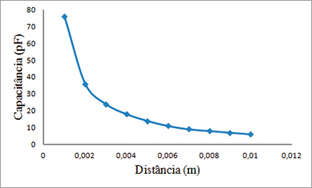
\includegraphics{img/cidepe-cxd.jpg}
	\caption{$C \times d$. Fonte: Cidepe.}
	\label{fig:imagem1}
\end{figure}

\begin{figure}[H]
	\centering
	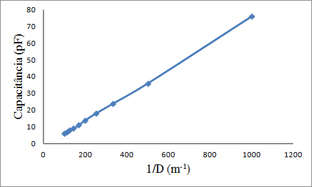
\includegraphics{img/cidepe-cx1d.jpg}
	\caption{$C \times 1/d$. Fonte: Cidepe.}
	\label{fig:imagem1}
\end{figure}

\textbf{Dicas}[B]

A capacitância é a principal propriedade de um capacitor, e diz respeito à capacidade de armazenamento das cargas elétricas. Podemos definir Capacitância como sendo a relação entre a quantidade de cargas acumuladas e a diferença de potencial aplicada às armaduras em um capacitor. Quanto maior a capacitância, maior a quantidade de cargas elétricas que podem ser armazenadas no dispositivo.


A capacitância é medida em uma unidade denominada Farad (batizada em homenagem ao célebre físico e químico Michael Faraday), abreviada pela letra F, e no geral os capacitores utilizam submúltiplos dessa unidade, pois a capacitância de 1 F é um valor muito elevado. Um capacitor de 1F conectado a uma fonte que forneça 1V de tensão elétrica irá armazenar uma carga de 1C, que equivale a 6,24 x 1018 elétrons.

As principais unidades utilizadas para representar a capacitância de um capacitor são as seguintes:

	%tabela 5
	\begin{table}[H]
		\centering
	\begin{tabular}{l|c|c}
		\hline 
		Nome da Unidade & Símbolo & Valor equivalente em Farads\\ 
		\hline 
		Milifarad & $m F$ & $1 \times 10^{-3}\,F$ \\ 
		Microfarad & $\mu F$ & $1 \times 10^{-6}\,F$ \\  
		Nanofarad & $n F$ & $1 \times 10^{-9}\,F$ \\  
		Picofarad & $p F$ & $1 \times 10^{-12}\,F$ \\ 
		\hline 
	\end{tabular} 
		\caption{Principais unidades de Capacitância}
		\label{tab:capacitancias}
	\end{table}

Um capacitor possui capacitância de um Farad quando uma carga elétrica de um Coulomb é armazenada em suas armaduras por uma tensão elétrica de um Volt. A capacitância é sempre um valor positivo.

\bibliographystyle{plain}
  \begin{thebibliography}{1}
    \bibitem{item-1} INSTITUTO DE FÍSICA GLEB WATAGHIN. “Aula 5: Capacitância”. Disponível em
<http://midia.cmais.com.br/assets/file/original/bc19adc4984d1dd3d06412d78fe66d166e7c3514.
pdf/>. Acesso em 12 de Julho de 2018.
    \bibitem{item-2} REDAÇÃO. “Resumo de física: Capacitância e tensão elétrica”. Disponível em
<https://guiadoestudante.abril.com.br/estudo/resumo-de-fisica-capacitancia-e-tensao-
eletrica/>. Acesso em 12 de Julho de 2018.
    \bibitem{item-3} BOSONTREINAMENTOS. "Treinamentos em Ciência e Tecnologia". Disponível em <http://www.bosontreinamentos.com.br/eletronica/curso-de-eletronica/especificacoes-dos-capacitores/>. Acesso em 25 de outubro de 2020.
    \bibitem{item-4} PLATO. "Ruptura Dielétrica". <http://plato.if.usp.br/~fge0211n/Main_Site/Extras/Extras_files/Ruptura%20diele%CC%81trica.pdf>. Acesso em 25 de outubro de 2020.
  \end{thebibliography}
%\noindent \texttt{V: 04-11-2022 11:33:00}

\section*{Experimento: - LEI DE OHM}
\section*{Teoria}

A aplicação de uma diferença de potencial elétrico V em um fio faz aparecer, nele, uma \textbf{corrente elétrica $I$}. A \textbf{resistência elétrica $R$} entre dois pontos quaisquer de um condutor é definida pela equação
\begin{equation}
    R = \frac{V}{I}
    \label{eq:R}
\end{equation}

\noindent A resistência $R$ é uma característica do fio como um todo, ou seja, depende do comprimento, da espessura e do material de que ele é feito. Por outro lado, a grandeza \textbf{resistividade ($\rho$)} é uma propriedade {\color{red}específica dos materiais} e depende de características microscópicas intrínsecas. Ou seja, pode-se lidar com fios de diferentes tamanhos e espessuras de um mesmo metal, cada um deles apresentando um valor diferente de resistência, porém, com a mesma resistividade. Essa grandeza informa como é a resposta microscópica do meio, ou seja, qual é a \textbf{densidade de corrente $J$} quando o meio é sujeito a um \textbf{campo elétrico $E$}. Matematicamente, tem-se esta relação microscópica:
\begin{equation}
    \rho = \frac{E}{J}
    \label{eq:rho}
\end{equation}

\noindent Como, no Sistema Internacional de Unidades (SI) as unidades de $E$ são $[V/m]$ (Volt/metro) e de $J$ são $[A/m^{2}]$ (Ampère/metro quadrado), $\rho$ é dado em $[\Omega.m]$ (ohm x metro).
No caso de um fio uniforme de comprimento $l$ e seção reta de área $A$, tem-se
\begin{equation}
    E = \frac{V}{l} \;\;\; \text{e} \;\;\; J = \frac{I}{A}
    \label{eq:EeJ}
\end{equation}

\noindent 
Combinando-se as equações \ref{eq:R}, \ref{eq:rho} e \ref{eq:EeJ}, chega-se a uma relação entre a resistência e a resistividade de um fio uniforme, dada por 
\begin{equation}
    R = \rho \frac{l}{A}
\end{equation}


\noindent Medindo-se a resistência de um fio uniforme e homogêneo em função de seu comprimento, pode-se determinar a resistividade do material de que ele é feito. Para isso, basta conhecer a área da seção reta do fio.


\section*{Prática}
	\section{Objetivos}
	
	Verificar experimentalmente a dependência da resistência em função dos seguinte parâmetros: A relação entre a voltagem aplicada  e acorrente; O Tipo de material, comprimento do fio, espessura do fio. 
	\section{Material utilizado}
	
	\begin{itemize}
		\item[a)] Fonte de Tensão e Corrente Contínua (CC);
		\item[b)] Uma Tábua didática Azheb - Lei de Ohm;
		\item[c)] Um multímetro;
		\item[d)] Dois fios ou cabos condutores;
		\item[e)] Um papel milimetrado;
		\item[f)] Uma régua ou trena ou paquímetro ou micrômetro.
		
	\end{itemize}

	\section{Procedimento experimental}
	
	\subsection{A - Relação entre a voltagem e a intensidade da corrente elétrica de um resistor}

\begin{enumerate}	
\item Monte o circuito de acordo com a figura \ref{fig:circuito-r-cc};

\begin{figure}[H]
\centering
    \begin{circuitikz}[american voltages]
    \draw %é (x1,y1) to [battery1, v=$V$] (x2,y2) uma matriz com origem no canto inferior esquerdo
      (0,0) to [battery1, v=$V$] (4,0)
      (0,2) to [ammeter, i=$I$] (4,2)
      (4,0) --  (4,2) 
      (0,0) to [R, color=red, R=$R$] (0,2)
      (-2,0) to [voltmeter, color=blue] (-2,2)
      (-2,0) --  (0,0)
      (-2,2) --  (0,2);  
    \end{circuitikz}
	\caption{Circuito CC Resistivo Básico. \textit{Fonte: Autor}.}
	\label{fig:circuito-r-cc}
\end{figure}

\item Ajuste o multímetro para atuar como amperímetro na escala para 10 A;

\item Monte o circuito, conforme o esquema da figura \ref{fig:circuito-r-cc}, com um fio de 1 m do painel, a fonte e o amperímetro (em série);  

\item Use os controles da fonte e varie a tensão entre $1\,V$ e $5\,V$, meça os valores de corrente e complete a Tabela \ref{tab:v-x-i}. {\color{red} \textsc{FAÇA AS MEDIDAS RAPIDAMENTE, PARA NÃO DANIFICAR A FONTE}};
\item Com os dados da Tabela, faça o gráfico $I \times V$. 

\item Analise o gráfico para determinar o tipo de função;

\item Qual a relação entre as grandezas envolvidas? 

\item Determine o valor médio de $V/I$;

\item Compare o erro entre o valor médio experimental calculado e o valor medido com o multímetro? 

\item Que significado físico tem $V/I$ ?

\end{enumerate}


	
	%Tabela 1
		\begin{table}[H]
			\centering
		\begin{tabular}{*{3}{|c}|}
			\hline 
			Tensão da fonte [$V$] & Corrente medida [$A$] & Cálculo $V/I \; [V/A]$\\ 
			\hline 
			1,0 & & \\ 
			\hline 
			2,0 & & \\ 
			\hline 
			3,0 & & \\ 
			\hline
			4,0 & & \\ 
			\hline 
			5,0 & & \\ 
                \hline  \hline 
			\multicolumn{2}{|r|}{\textbf{Media:}} & \\ 
				\hline 		
		\end{tabular}
			\caption{\label{tab:v-x-i} Razão entre Voltagem e Corrente em condutor.}
		\end{table}
	
	
	\subsection{B - Dependência de R em relação ao comprimento do fio}
    
    \begin{enumerate}	
	\item Monte o circuito de acordo com a figura \ref{fig:circuito-r2-cc};

\begin{figure}[H]
	\centering
    \begin{circuitikz}[american voltages]
    \draw
      (0,0) to [battery2, v=$V$] (4,0)
      (0,2) to [ohmmeter] (4,2)
      (4,0) --  (4,2) 
      (0,0) to [vR, color=red, vR=$R$] (0,2);
    \end{circuitikz}
	\caption{Circuito CC Resistivo Variável Básico. \textit{Fonte: Autor}.}
	\label{fig:circuito-r2-cc}
\end{figure}
	

    \item Ajuste o multímetro para atuar como ohmímetro;
    \item Para \textbf{um} fio do painel, conecte o multímetro e meça as diferentes resistências para diferentes comprimentos;  
    \item Anote os valores na Tabela \ref{tab:RxL};
    \item Com os dados da Tabela \ref{tab:RxL}, faça o gráfico $R \times L$;  
    \item Analise o gráfico para determinar o tipo de função;
    \item Qual a relação entre as grandezas envolvidas?
    \end{enumerate}
 
%Tabela 2
		\begin{table}[H]
			\centering
		\begin{tabu}{| X[c] | X[c] | X[c] | X[c] |}
			\hline 
			Condutor resistivo utilizado (material) e diâmetro $\oslash$(mm) &  Comprimento do fio $(m)$ & Resistência ôhmica medida  $(\Omega)$ & Quociente  $(R.A/L)$ \\ %cabeçalho
			\hline 
			Ni-Cr $\oslash \;0,36$& 0,20 &  &    \\ 
			\hline 
			Ni-Cr $\oslash \;0,36$ & 0,40 &  &    \\ 
			\hline 
			Ni-Cr $\oslash \;0,36$ & 0,60 &  &    \\ 
			\hline 
			Ni-Cr $\oslash \;0,36$ & 0,80 &  &    \\ 
			\hline 
			Ni-Cr $\oslash \;0,36$ & 1,00 &  &    \\ 
			\hline \hline 
			\multicolumn{3}{|r| }{\textbf{Média:}} & \\
			\hline 
		\end{tabu} 
			\caption{Variação da resistência em função do comprimento de um condutor $R/L$.}
			\label{tab:RxL}
		\end{table} 
  
\subsection{D - Dependência de R em relação à área da seção reta do condutor  }

\begin{enumerate}
    \item Complete a Tabela \ref{tab:RxA} abaixo para fios \textbf{com $L=1\,m$} e com diferentes materiais e áreas de seção transversal.
    \item Com os dados da Tabela \ref{tab:RxA}, faça o gráfico R x A.
    \item Analise o gráfico para determinar o tipo de função.
    \item Qual a relação entre as grandezas envolvidas?
\end{enumerate}
        
        %Tabela 3
		\begin{table}[H]
			\centering
		\begin{tabu}{| X[c] | X[c] | X[c] | X[c] |}
			\hline 
			Condutor (material) e diâmetro $\oslash \;$(m) &  Área da seção transversal $(m^{2})$ & Resistência ôhmica medida  $(\Omega)$ & Produto calculado (RxA)  \\ %cabeçalho
			\hline 
			 Ni-Cr $\oslash \;3,6 \times 10^{-4}$&  &  &    \\ 
			\hline 
			 Ni-Cr $\oslash \;5,1 \times 10^{-4}$&  &  &    \\ 
			\hline 
			 Ni-Cr $\oslash \;7,2 \times 10^{-4}$&  &  &    \\ 
			\hline
			 Fe $\oslash \;5,1 \times 10^{-4}$&  &  &    \\ 
			\hline 
		\end{tabu} 
			\caption{Variação da resistência em função do diâmetro de um condutor $R \times A$.}
			\label{tab:RxA}
		\end{table} 

    \subsection{C - Resistividade}

\begin{enumerate}
    \item Complete a Tabela \ref{tab:resistividade} abaixo para fios de mesmo material (Ni-Cr) com diferentes áreas de seção transversal (\textbf{copie da Tabela \ref{tab:RxA}});
    \item Calcule a média e compare com os valores da literatura.
\end{enumerate}    
    
    		%Tabela 4
		\begin{table}[H]
			\centering
		\begin{tabular}{|c|c|c|l|}
			\hline 
			Diâmetro $\oslash \; (m)$ & Área $[m^2]$ &  Resistência $(\Omega)$ & Resistividade $(\rho)\,[\Omega .m]$ \\ 
			\hline 
			Ni-Cr $3,6 \times 10^{-4}$ &  &  & \\ 
			\hline 
			Ni-Cr $5,1 \times 10^{-4}$ &  &  & \\ 
			\hline 
			Ni-Cr $7,2 \times 10^{-4}$ &  &  & \\ 
			\hline \hline 
			\multicolumn{3}{|r| }{\textbf{Média:}} & \\
			\hline 
		\end{tabular}
			\caption{Coeficiente de resistividade para o Nicromo (Ni-Cr)}
			\label{tab:resistividade}
		\end{table} 
		




\section{Relatório ou Exercícios}

\begin{itemize}
\item Construa o relatório apresentando os itens obrigatórios. 

\item Comente as prováveis fontes de erro. 

\item Responda as questões formuladas. 

\item Apresente os dados organizados em Tabelas. 

\item Apresente a análise dos dados e gráficos. 

\item Apresente os resultados solicitados no sistema internacional de unidades com todos os cálculos efetuados.  
	
\end{itemize}

\noindent
{\color{red} \rule{\linewidth}{0.5mm} }
\textbf{Dica:}

\noindent \texttt{ O que se espera? Algo do tipo...}


\begin{figure}[H]
	\centering
	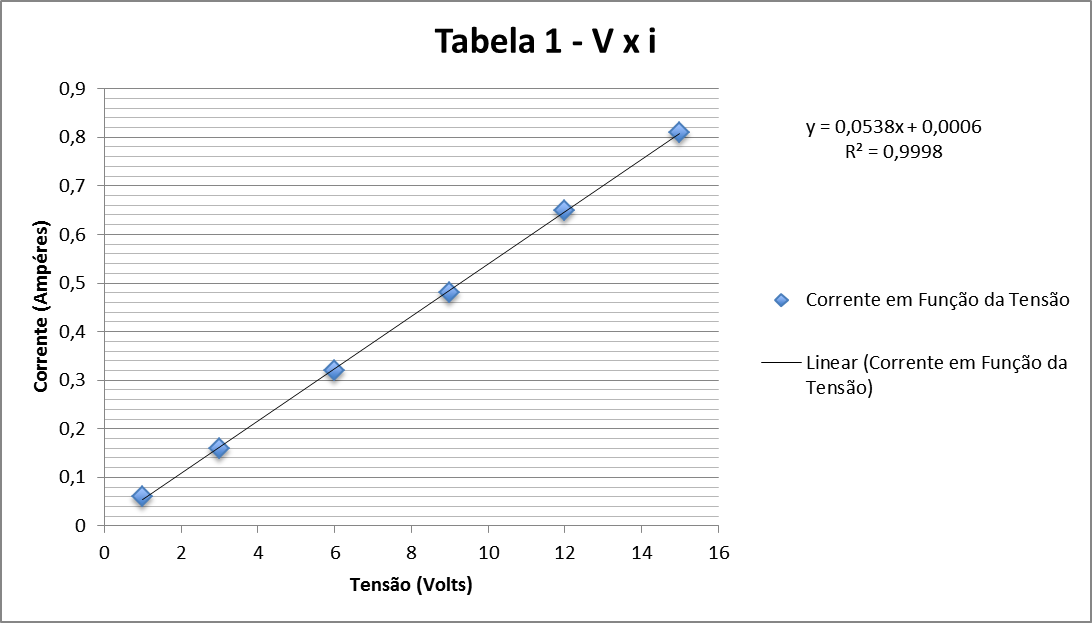
\includegraphics[scale=.4]{img/lei-de-ohm.jpg}
	\caption{$I \times V$. Fonte: Web.}
	\label{fig:imagem1}
\end{figure}

\noindent Coeficientes de Resistividade:

\noindent $\rho_{Ni-Cr} = 10,0 \times 10^{-7}\;\Omega.m$

\noindent $\rho_{Fe} = 10,0 \times 10^{-8}\;\Omega.m$







%\noindent \texttt{V: 25-10-2022 17:28:00}
\section*{Experimento: - CAPACITÂNCIA}
	\section{Objetivos}
	
	Estudar o efeito capacitivo entre as placas de um capacitor variável de placas paralelas - Figura \ref{fig:cidepe-capacitor}, verificando a relação da capacitância $C=\epsilon_{0} A/d$ em função da distância $d$ entre as placas; Medir a constante de permissividade ${\epsilon}_{0}$ e medir a constante dielétrica de distintos materiais isolantes como papel, \href{https://pt.wikipedia.org/wiki/Espuma_vin\%C3\%ADlica_acetinada}{ E.V.A (\textit{Ethylene Vinyl Acetate})} e isopor.	
	\section{Material utilizado}
	
\begin{wrapfigure}{r}{0.7\textwidth}
    \centering
    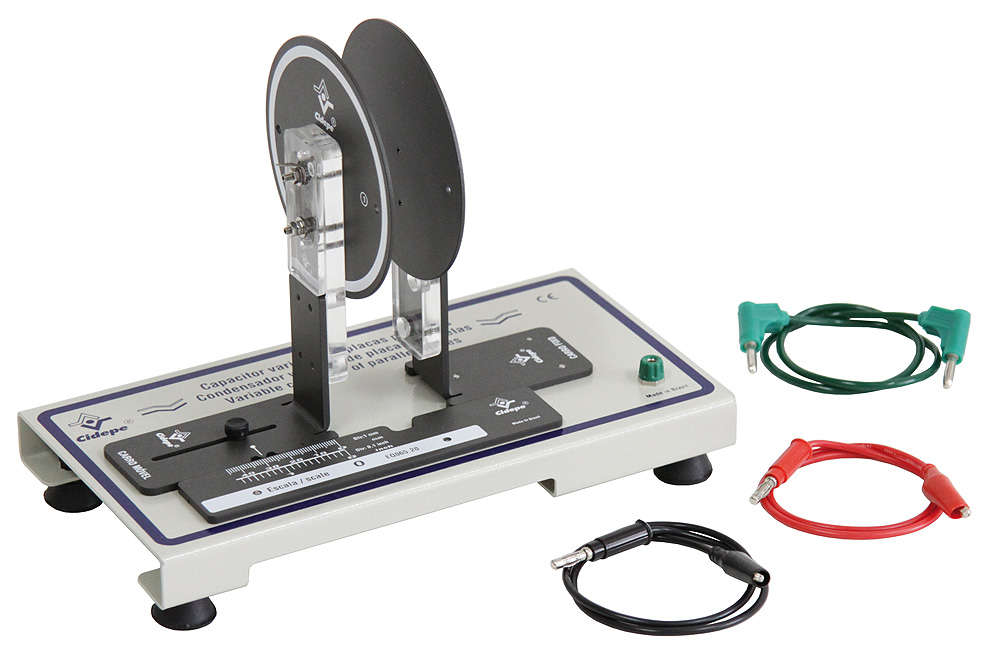
\includegraphics[width=.36\textwidth]{img/cidepe-capacitor.jpg}
    \caption{Capacitor de placas paralelas com separação variável montado em isolante acrílico. \textit{Fonte: Cidepe}.}
    \label{fig:cidepe-capacitor}
\end{wrapfigure}
	
	\begin{itemize}
		\item[a)] Um capacitor variável de placas paralelas: 2,3 pF - 280 pF;
		\item[b)] Um medidor digital de capacitância;
		\item[c)] Dois fios ou cabos condutores;
		\item[d)] Um papel milimetrado;
		\item[e)] Folhas de papel ou papelão;
		\item[f)] Lâminas de isolantes E.V.A, EPS (Isopor), Vidro, Acrílico,etc;
		\item[j)] Uma régua ou trena ou paquímetro.
		
	\end{itemize}
	
\begin{comment}
\begin{figure}[H]
	\centering
	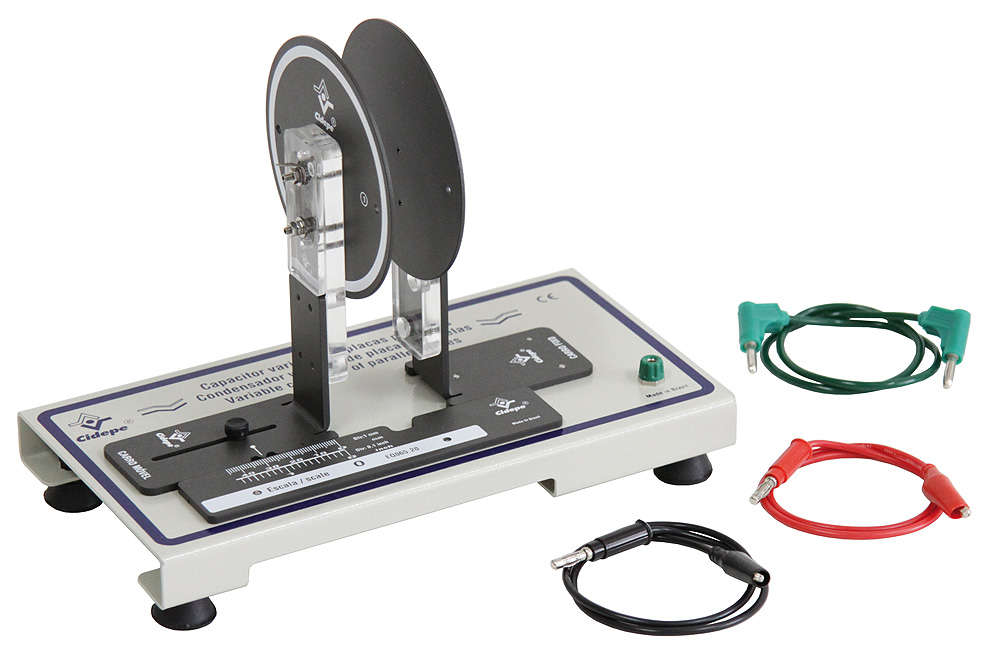
\includegraphics[scale=.3]{img/cidepe-capacitor.jpg}
	\caption{Capacitor de placas paralelas com separação variável montado em isolante acrílico. Fonte: Cidepe.}
	\label{fig:imagem1}
\end{figure}
\end{comment}


\section{Fundamentos teóricos}
	
	Se preenchermos o espaço entre as placas de um capacitor com um dielétrico (isolante), o que acontecerá com a capacitância? \textbf{Michel Faraday} (1791-1867) investigou este assunto pela primeira vez em 1837. Usando equipamento simples, ele descobriu que a capacitância aumentava por um fator $\kappa$, que ele chamou de constante dielétrica do material isolante. Outro efeito importante na introdução do dielétrico no capacitor é limitar a diferença de potencial que se pode aplicar entre as placas a um certo valor ${V}_{max}$, chamado de potencial de ruptura. Se este valor for excedido, o material dielétrico se romperá e formará um caminho condutor ({\color{red}\textbf{arco elétrico}}) entre as placas. Logo, todo material dielétrico possui uma rigidez dielétrica característica, que é o valor máximo do campo elétrico que um isolante pode tolerar sem se romper e se tornar um condutor (para o ar a rigidez dielétrica é $~3\times10^{6} \,V.m^{-1}$, ou seja tensões ou diferenças de potencial ${V}_{max}$ acima desses valores, permitem a ocorrência de um \textbf{arco elétrico} ou popularmente \textit{raio/faísca/centelha}). Na Tabela \ref{tab:rigidez-materiais} são mostradas algumas constantes dielétricas importantes.
	
	%tabela 1
	\begin{table}[H]
		\centering
	\begin{tabular}{l|c|c}
		\hline 
		Material & Constante Dielétrica, $\kappa$ & Rigidez Dielétrica $E_{max} (10^{6}\,V.m^{-1})$ \\ 
		\hline 
		Ar(1 atm) & 1,0006 & 3 \\ 
        Madeira & & 10 \\
        Borracha & & 12 \\
	Papel & 3,5 & 16 \\ 
        Poliéster & 3,6 & 21,7 \\ 
        Vidro & & 30 \\
        Mica & & 60 \\
        Teflon & & 80 \\
        
		\hline 
	\end{tabular} 
		\caption{Constante dielétrica e rigidez dielétrica}
		\label{tab:rigidez-materiais}
	\end{table}

	\section{Procedimento experimental}
	
	\subsection{A - MEDIDA DA PERMISSIVIDADE ELÉTRICA ($\epsilon_{0}$)}
	
	\begin{itemize}
		\item[a)] Certifique-se de que o capacitor esteja descarregado, fazendo contato entre as duas placas por meio de um fio ou cabo condutor;
		\item[b)] Meça o diâmetro, calcule o raio e com este a área das placas do capacitor (use: $A=\pi r^2$, onde $r$ é o \textbf{raio} das placas). Anote os resultados na Tabela \ref{tab:area-placas};
		
		%tabela 2
		\begin{table}[H]
			\centering
		\begin{tabular}{|c|c|}
			\hline 
			Diâmetro das Placas ($m$) & Área das Placas do Capacitor ($m^2$)\\ 
			\hline
			&  \\ 
			\hline 
		\end{tabular}
			\caption{\label{tab:area-placas} Diâmetro e área do capacitor}
		\end{table}
		
		\item[c)] Fazer a conexão do medidor de capacitância nas placas do capacitor. \textbf{Zerar o aparelho antes de fazer a medida};
		\item[d)] Com a chave seletora do medidor em 200 pF, estabeleça um espaçamento aproximado de 1,0 ou 10 mm entre as placas do capacitor. Anote o valor da capacitância $C_{exp}$ na Tabela \ref{tab:cte-dieletrica}; 
		\item[e)] Calcule a constante de permissividade (use a relação: $ \epsilon_{0}= C_{exp} \, d / A. \kappa_{ar} $). Anote o resultado na Tabela \ref{tab:cte-dieletrica};
		\item[f)] Calcule o erro experimental, entre o valor teórico (da literatura), e o valor experimental (medido). Anote o resultado na Tabela \ref{tab:cte-dieletrica}. 
	
		%tabela 3
		\begin{table}[H]
			\centering
		\begin{tabular}{|c|c|c|c|c|}
			\hline 
			$C_{exp}$ (pF) & $\epsilon_{0}$ (Teórico)(pF) & $\epsilon_{0}$ (experimental)(pF) & Erro (Absoluto) & Erro (\%)  \\ 
			\hline 
			& 8,85 & & & \\ 
			\hline 
		\end{tabular}
			\caption{Medição da constante dielétrica}
			\label{tab:cte-dieletrica}
		\end{table} 
	\end{itemize}
	
	\subsection{B - VARIAÇÃO DA CAPACITÂNCIA COM A SEPARAÇÃO ENTRE AS PLACAS}
	
	\begin{itemize}
		\item[a)] Certifique-se de que o capacitor esteja descarregado;
		\item[b)] Com a chave seletora do medidor em 200 pF, varie a distância entre as placas de 1 mm em 1 mm até 10 mm (5 mm em 5 mm até 50 mm no Capacitor \href{https://www.cidepe.com.br/index.php/br/produtos-interna/capacitor-variavel-de-placas-paralelas-e-cabos-0-a-255-pf-1875}{Cidepe EQ065D} ou similar). Para cada variação meça a capacitância correspondente ({\color{red}\textbf{Para uma melhor precisão, a partir da segunda medida selecione a posição da chave em $200 \,\mu F$}}). Anote os valores das capacitâncias $ C_{exp} $ na Tabela \ref{tab:c-versus-inv-d};

		%tabela 4
		\begin{table}[H]
			\centering
		\begin{tabu}{| l | X[c] | X[c] | X[c] | X[c] | X[c] | X[c] | X[c] | X[c] | X[c] | X[c] |}
			\hline 
			d ($mm$) &  &  &  &  &  &  &  &  &  &  \\ 
			\hline 
			$C_{exp} \,(pF$) &  &  &  &  &  &  &  &  &  &  \\ 
			\hline 
			1/d ($mm^{-1}$) &  &  &  &  &  &  &  &  &  &  \\ 
			\hline 
		\end{tabu} 
			\caption{Variação da capacitância em função de d e 1/d}
			\label{tab:c-versus-inv-d}
		\end{table} 
	
		\item[c)] Faça um gráfico, digital ou em papel milimetrado, de $ C_{exp} \times d $ e em seguida de $ C_{exp} \times (1/d) $;
		\item[d)] Obtenha o coeficiente angular \textbf{$\alpha$} da reta $ C_{exp} \times (1/d) $ e compare com o valor do produto $ \kappa_{ar} \epsilon_{0} A$. Anote os valores na Tabela \ref{tab:coeficientes}; 
		\item[e)] Calcule o erro experimental absoluto e percentual.
		
		%tabela 5
		\begin{table}[H]
			\centering
		\begin{tabular}{|c|c|c|c|}
			\hline 
			Coeficiente angular $\alpha$ (pF.m) & $\kappa_{ar} \epsilon_{0} A$ (Teórico)(pFm) & Erro (Absoluto) & Erro (\%) \\ 
			\hline 
			&  &  & \\ 
			\hline 
		\end{tabular}
			\caption{Coeficientes e constantes}
			\label{tab:coeficientes}
		\end{table} 
		
	\end{itemize}
	
	\subsection{C - MEDIDAS DAS CONSTANTES DIELÉTRICAS DOS ISOLANTES}
	
	\begin{itemize}
		\item[a)] Certifique-se de que o capacitor esteja descarregado;
		\item[b)] Escolher uma placa/isolante dielétrico, folha de papel. Em seguida, medir sua espessura com um paquímetro (ou um micrômetro);
		\item[c)] Meça a capacitância do ar $C_{ar}$, para uma separação miníma entre as placas, aproximadamente ~1 mm (ou ~10mm no \href{https://www.cidepe.com.br/index.php/br/produtos-interna/capacitor-variavel-de-placas-paralelas-e-cabos-0-a-255-pf-1875}{Cidepe EQ065D} ou similar) com o medidor ({\color{red}\textbf{selecione uma escala de 200 pF}});
		\item[d)] Insira o dielétrico entre as placas do capacitor, em uma posição firme, e meça a capacitância equivalente, ${C}_{d+ar}$ com o medidor ({\color{red}\textbf{selecione uma escala de $200 \,\mu F$}}). \hbox{\textbf{Obs: $C_{d}$ = capacitância com dielétrico}};
		
		\item[e)] Calcule a capacitância da placa dielétrica usando a relação: $ 1/C_{placa}=1/C_{d+ar}-1/C_{ar}$. Anote o valor na Tabela \ref{tab:cte-dieletrica-isolantes};
		\item[f)] Calcule a constante dielétrica do isolante, $ \kappa_{isolante}=C_{d}.d{/\epsilon_{0}A}$;
		\item[g)] Calcule erro experimental entre as constantes teórica (literatura) e experimental;
			\item[h)] Repita os passos a-g para os outros isolantes.
		
		%tabela 6
		\begin{table}[H]
		\centering
		\begin{tabular}{|c|c|c|c|c|c|c|c|}
			\hline 
			$d$ (mm) & $C_{ar}$ (pF) & $C_{d+ar}$ (pF) & $\kappa_{isolante}$ (teórico) &  $\kappa_{isolante}$ (exp.) & \|Erro\|  & Erro (\%) \\ 
			\hline 
			&  &  &  &  &  &\\ 
			\hline 
		\end{tabular} 
			\caption{Constante dielétrica dos isolantes}
			\label{tab:cte-dieletrica-isolantes}
		\end{table}
	\end{itemize}

\section{Exercícios}

\begin{itemize}
	\item[a)] Justifique os erros observados no experimento;
	
	\item[b)] Qual o valor da constante de permissividade elétrica? Use os dados experimentais;

	\item[c)] Quais são os valores das constantes dielétricas? Use os dados experimentais;
	
	\item[d)] Para um potencial constante, a carga do capacitor aumenta ou diminui com a introdução do dielétrico? Justifique;
	
	\item[e)] Qual a finalidade do dielétrico no capacitor? Justifique.
	
\end{itemize}

\noindent{\color{red} \rule{\linewidth}{0.5mm} }\textbf{Desafio:}
Considere - Capacitor com dielétrico
\\
\textit{Será que conseguimos realizar um experimento mostrando o potencial $V$ antes e após a introdução deum material dielétrico em um capacitor didático de placas planas?}

\noindent
\textsc{Hipótestes}

Sabe-se empiricamente que a capacitância aumenta quando o capacitor é preenchido com um material dielétrico. Os primeiros a constatarem isto foram (independentemente) Faraday (1837) e Cavendish (1773). Todo dielétrico pode ser caracterizado por uma grandeza denominada \textbf{constante dielétrica}, denotada pela letra grega $\kappa$, definida por :
 $$\kappa = \frac{C}{C_0}$$
Onde $C$ e ${C_0}$ são as capacitâncias de um mesmo capacitor respectivamente com e sem dielétrico. Note que o valor mínimo $k = 1$ ocorre no caso em que o capacitor está vazio, ou seja, $ C = C_0$ O valor de $\kappa$ a temperatura de 25°C é 1,00059 para o ar, 2,25 para a parafina, 78,2 para água destilada. 
Quando um capacitor é carregado com carga $Q$ e mantido isolado, de tal forma que sua carga não pode variar, a mudança da capacitância deve ser acompanhada de uma mudança do potencial entre as placas. De fato, como $Q=C.V$ não muda, então:

$$C_0 \, V_0 = C\,V,$$

\noindent
em que $V_0$ e $V$ são os potenciais respectivamente antes e depois da introdução do dielétrico. Portanto, o novo potencial:

$$V = \frac{C_0}{C}V_0=\frac{1}{\kappa}V_0$$

\noindent
diminui por um fator $\kappa^{-1}$ em relação ao potencial $V_0$ , na ausência do dielétrico. {\color{purple}\textbf{\textit{prove isso}} }

\hskip

\noindent{\color{red} \rule{\linewidth}{0.5mm} }
\textbf{Dicas}[A]

\noindent \texttt{ O que se espera?}


\begin{figure}[H]
	\centering
	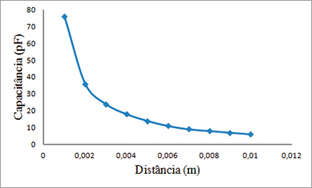
\includegraphics{img/cidepe-cxd.jpg}
	\caption{$C \times d$. Fonte: Cidepe.}
	\label{fig:imagem1}
\end{figure}

\begin{figure}[H]
	\centering
	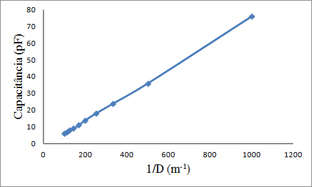
\includegraphics{img/cidepe-cx1d.jpg}
	\caption{$C \times 1/d$. Fonte: Cidepe.}
	\label{fig:imagem1}
\end{figure}

\textbf{Dicas}[B]

A capacitância é a principal propriedade de um capacitor, e diz respeito à capacidade de armazenamento das cargas elétricas. Podemos definir Capacitância como sendo a relação entre a quantidade de cargas acumuladas e a diferença de potencial aplicada às armaduras em um capacitor. Quanto maior a capacitância, maior a quantidade de cargas elétricas que podem ser armazenadas no dispositivo.


A capacitância é medida em uma unidade denominada Farad (batizada em homenagem ao célebre físico e químico Michael Faraday), abreviada pela letra F, e no geral os capacitores utilizam submúltiplos dessa unidade, pois a capacitância de 1 F é um valor muito elevado. Um capacitor de 1F conectado a uma fonte que forneça 1V de tensão elétrica irá armazenar uma carga de 1C, que equivale a 6,24 x 1018 elétrons.

As principais unidades utilizadas para representar a capacitância de um capacitor são as seguintes:

	%tabela 5
	\begin{table}[H]
		\centering
	\begin{tabular}{l|c|c}
		\hline 
		Nome da Unidade & Símbolo & Valor equivalente em Farads\\ 
		\hline 
		Milifarad & $m F$ & $1 \times 10^{-3}\,F$ \\ 
		Microfarad & $\mu F$ & $1 \times 10^{-6}\,F$ \\  
		Nanofarad & $n F$ & $1 \times 10^{-9}\,F$ \\  
		Picofarad & $p F$ & $1 \times 10^{-12}\,F$ \\ 
		\hline 
	\end{tabular} 
		\caption{Principais unidades de Capacitância}
		\label{tab:capacitancias}
	\end{table}

Um capacitor possui capacitância de um Farad quando uma carga elétrica de um Coulomb é armazenada em suas armaduras por uma tensão elétrica de um Volt. A capacitância é sempre um valor positivo.

\bibliographystyle{plain}
  \begin{thebibliography}{1}
    \bibitem{item-1} INSTITUTO DE FÍSICA GLEB WATAGHIN. “Aula 5: Capacitância”. Disponível em
<http://midia.cmais.com.br/assets/file/original/bc19adc4984d1dd3d06412d78fe66d166e7c3514.
pdf/>. Acesso em 12 de Julho de 2018.
    \bibitem{item-2} REDAÇÃO. “Resumo de física: Capacitância e tensão elétrica”. Disponível em
<https://guiadoestudante.abril.com.br/estudo/resumo-de-fisica-capacitancia-e-tensao-
eletrica/>. Acesso em 12 de Julho de 2018.
    \bibitem{item-3} BOSONTREINAMENTOS. "Treinamentos em Ciência e Tecnologia". Disponível em <http://www.bosontreinamentos.com.br/eletronica/curso-de-eletronica/especificacoes-dos-capacitores/>. Acesso em 25 de outubro de 2020.
    \bibitem{item-4} PLATO. "Ruptura Dielétrica". <http://plato.if.usp.br/~fge0211n/Main_Site/Extras/Extras_files/Ruptura%20diele%CC%81trica.pdf>. Acesso em 25 de outubro de 2020.
  \end{thebibliography}

\end{document}